\documentclass[a4paper]{book}
\usepackage[left=2.00cm, right=2.00cm, top=2.50cm, bottom=2.00cm]{geometry}

\usepackage{amsmath,amssymb}
\usepackage{graphicx}
\usepackage{color}
\definecolor{bl}{gray}{0.9}

% figure position
\usepackage{booktabs}
\usepackage{here}

\title{Note: The Elements of Computing Systems}

\begin{document}
\maketitle

\chapter*{Preface}
This is my study note for The Elements of Computing Systems (ISBN:  978-0262640688) by Noam Nisan and Shimon Schocken.

\chapter{Boolean Logic}
\textbf{Boolean Algebra}
\begin{align*}
    x ~\mathrm{or}~ y & = \bar{x}y + x\bar{y} + xy \\
    &                   = \bar{x}y + x(y + \bar{y}) \\
    &                   = x + \bar{x}y \\
    &                   = x + \overline{ x + \bar{y} } \\
    &                   = \overline{ \overline{ x + \overline{(x + y) } } } \\
    &                   = \overline{\bar{x} (x + \bar{y} ) } \text{~ ~ ~ where } \overline{x + y} = \bar{x} \bar{y} \\
    &                   = \overline{ x\bar{x} + \bar{x}\bar{y} } \\
    &                   = \overline{ \bar{x} \bar{y} } \\
    &                   = \overline{\overline{x + y}} \\
    &                   = x + y \\
%
%
    \text{if } y \text{ then } x & = \bar{x}\bar{y} + x \bar{y} + xy \\
    &                              = \bar{x}\bar{y} + x(y + \bar{y}) \\
    &                              = x + \bar{x}\bar{y} \\
    &                              = x + \overline{x + y} \\
    &                              = \overline{ \overline{ x + \overline{x + y} } } \\
    &                              = \overline{ \bar{x}(x + y) } \\
    &                              = \overline{ x\bar{x} + \bar{x}y } \\
    &                              = \overline{ \bar{x}y } \\
    &                              = x + \bar{y} \\
%
%
    \text{if } x \text{ then } y & = \bar{x}\bar{y} + \bar{x}y + xy \\
    &                              = \bar{x}\bar{y} + (x + \bar{x}) y \\
    &                              = \bar{x}\bar{y} + y \\
    &                              = \overline{x + y} + y \\
    &                              = \overline{ \overline{ \overline{x + y} + y} } \\
    &                              = \overline{ (x + y) \bar{y} } \\
    &                              = \overline{ x\bar{y} + y\bar{y} } \\
    &                              = \overline{ x \bar{y} } \\
    &                              = \bar{x} + y \\
%
%
    x \text{ nand } y & = \bar{x}\bar{y} + \bar{x}y + x \bar{y} \\
    &                   = \bar{y}(x + \bar{x}) + \bar{x} y \\
    &                   = \bar{y} + \bar{x} y \\
    &                   = \bar{x} + \bar{y} \text{~ ~ ~ where } x + y    = x + \bar{x}y \\
    &                   = \overline{ \overline{ \bar{x} + \bar{y} } } \\
    &                   = \overline{ xy }
\end{align*}







\setcounter{chapter}{4}
%%%%%%%%%%%%%%%%%%%%%%%%%%%%%%%%%%%%%%%%%%%%
%%%%%%%%%%%%%%%%%%%%%%%%%%%%%%%%%%%%%%%%%%%%
\chapter{Computer Architecture}




\section{Memory}
\begin{figure}[H]
    \centering
    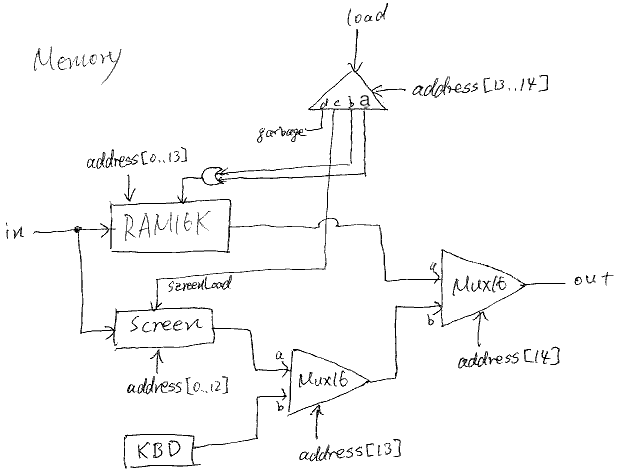
\includegraphics{pic/project05/memory.png}
    \caption{memory}
\end{figure}


\section{CPU}

$\text{C-instruction} = 111a c_1 c_2 c_3 c_4 c_5 c_6 d_1 d_2 d_3 j_1 j_2 j_3$

\begin{itemize}
    \item $d_1$: destination A
    \item $d_2$: destination D
    \item $d_3$: destination M
\end{itemize}


\begin{figure}[H]
    \centering
    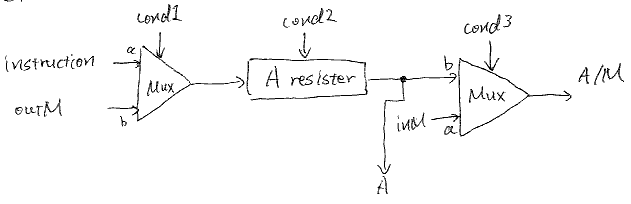
\includegraphics{pic/project05/cpu1.png}
    \caption{memory}
\end{figure}

\begin{align*}
    \text{cond1} & = \text{instruction}[15] \\
    \text{cond2} & = (\text{not } \text{instruction}[15]) \text{ or } (\text{instruction}[15] \text{ and } \text{instruction}[5]) \\
    \text{cond3} & = \text{instruction}[15] \text{ and } \text{ not } \text{instruction}[12]
\end{align*}

\begin{itemize}
    \item instruction[15]: opcode
    \item instruction[12]: C-instruction's $a$. If $a$ is $1$, comp includes A, otherwise, comp includes M.
    \item instruction[5]: destination A.
\end{itemize}


\begin{figure}[H]
    \centering
    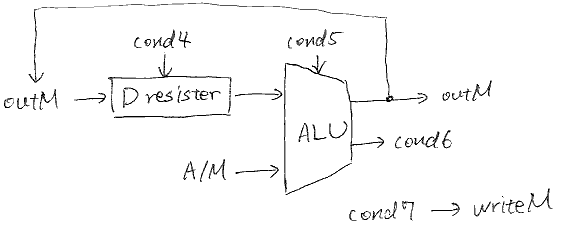
\includegraphics{pic/project05/cpu2.png}
    \caption{memory}
\end{figure}

\begin{align*}
    \text{cond4} & = \text{instruction}[15] \text{ and } \text{instruction}[4] \\
    \text{cond5} & = \begin{cases}
                        \text{zx} = \text{instruction}[11] = c_1 \\
                        \text{nx} = \text{instruction}[10] = c_2 \\
                        \text{zy} = \text{instruction}[9] = c_3 \\
                        \text{ny} = \text{instruction}[8] = c_4 \\
                        \text{f}  = \text{instruction}[7] = c_5 \\
                        \text{no} = \text{instruction}[6] = c_6
                    \end{cases} \\
    \text{cond6} & = (\text{zr}, \text{ng}) \\
    \text{cond7} & = \text{instruction}[15] \text{ and } \text{instruction}[3]
\end{align*}

\begin{itemize}
    \item \text{instruction}[3]: $d_3$, destination M
    \item \text{instruction}[4]: $d_2$, destination D
\end{itemize}



\begin{figure}[H]
    \centering
    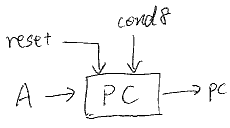
\includegraphics{pic/project05/cpu3.png}
    \caption{memory}
\end{figure}


\begin{align*}
    \text{cond8} = & \overline{\text{zr}} \cdot \overline{\text{ng}} \cdot \overline{j_1} \cdot \overline{j_2} \cdot \overline{j_3} \text{~~~~~~~ (JGT)} \\
                 & + \overline{\text{zr}} \cdot \overline{j_1} \cdot j_2 \cdot j_3 \text{~~~~~~ (JEQ)} \\
                 & + \overline{\text{ng}} \cdot \overline{j_1} \cdot j_2 \cdot j_3 \text{~~~~~~ (JGE)} \\
                 & + \text{ng} \cdot j_1 \cdot \overline{j_2} \cdot \overline{j_3} \text{~~~~~~ (JLT)} \\
                 & + \overline{\text{zr}} \cdot j_1 \cdot \overline{j_2} \cdot j_3 \text{~~~~~~ (JNE)} \\
                 & + (\text{zr} + \text{ng}) \cdot j_1 \cdot j_2 \cdot \overline{j_3} \text{~~~~~~ (JLE)} \\
                 & + j_1 \cdot j_2 \cdot j_3 \text{~~~~~~ (JMP)}
\end{align*}

 \setcounter{chapter}{6}
\chapter{Virtual Machine I: Stack Arithmetic}
\section{Arithmetic}

\[
    \texttt{add (sub)}
    \Rightarrow
    %
    \begin{cases}
        \texttt{ // SP--                            } \\
        \texttt{ @SP                                } \\
        \texttt{ M=M-1                              } \\
        \\
        \texttt{ // D = y                           } \\
        \texttt{ A=M                                } \\
        \texttt{ D=M                                } \\
        \\
        \texttt{ // SP--                            } \\
        \texttt{ @SP                                } \\
        \texttt{ M=M-1                              } \\
        \\
        \texttt{ // *SP = y + x (add) / x - y (sub) } \\
        \texttt{ A=M                                } \\
        \texttt{ M=D+M (add) / M=M-D (sub)          } \\
        \\
        \texttt{ // SP++                            } \\
        \texttt{ @SP                                } \\
        \texttt{ M=M+1                              }
    \end{cases}
\]

\[
    \texttt{neg, not}
    \Rightarrow
    %
    \begin{cases}
        \texttt{ // SP--                 } \\
        \texttt{ @SP                     } \\
        \texttt{ @M=M-1                  } \\
        \\
        \texttt{ // -M                   } \\
        \texttt{ A=M                     } \\
        \texttt{ M=-M (neg) / M=!M (not) } \\
        \\
        \texttt{ // SP++                 } \\
        \texttt{ @SP                     } \\
        \texttt{ M=M+1                   }
    \end{cases}
\]


\[
    \texttt{eq, gt, lt}
    \Rightarrow
    \begin{cases}
        ~ ~ ~ ~\texttt{ // SP--                             } \\
        ~ ~ ~ ~\texttt{ @SP                                 } \\
        ~ ~ ~ ~\texttt{ M=M-1                               } \\
        ~ ~ ~ ~\\
        ~ ~ ~ ~\texttt{ // D = y                            } \\
        ~ ~ ~ ~\texttt{ A=M                                 } \\
        ~ ~ ~ ~\texttt{ D=M                                 } \\
        ~ ~ ~ ~\\
        ~ ~ ~ ~\texttt{ // SP--                             } \\
        ~ ~ ~ ~\texttt{ @SP                                 } \\
        ~ ~ ~ ~\texttt{ M=M-1                               } \\
        ~ ~ ~ ~\\
        ~ ~ ~ ~\texttt{ // x - y                            } \\
        ~ ~ ~ ~\texttt{ A = M                               } \\
        ~ ~ ~ ~\texttt{ D=M-D                               } \\
        ~ ~ ~ ~\\
        ~ ~ ~ ~\texttt{ // if condition then -1 else 0 end  } \\
        ~ ~ ~ ~\texttt{ @then                               } \\
        ~ ~ ~ ~\texttt{ D;jEQ (eq),  D;JGT (gt), D:JLT (lt) } \\
        ~ ~ ~ ~\texttt{ @SP                                 } \\
        ~ ~ ~ ~\texttt{ A=M                                 } \\
        ~ ~ ~ ~\texttt{ M=0                                 } \\
        ~ ~ ~ ~\texttt{ @end                                } \\
        ~ ~ ~ ~\texttt{ 0;JMP                               } \\
        \texttt{ (then)                                     } \\
        ~ ~ ~ ~\texttt{ @SP                                 } \\
        ~ ~ ~ ~\texttt{ A=M                                 } \\
        ~ ~ ~ ~\texttt{ M=-1                                } \\
        \texttt{ (end)                                      } \\
        \\
        ~ ~ ~ ~\texttt{ // SP++                             } \\
        ~ ~ ~ ~\texttt{ @SP                                 } \\
        ~ ~ ~ ~\texttt{ M=M+1                               } \\
    \end{cases}
\]

\[
    \texttt{and, or}
    \Rightarrow
    \begin{cases}
        \texttt{ // SP--                  } \\
        \texttt{ @SP                      } \\
        \texttt{ M=M-1                    } \\
        \\
        \texttt{ // D = y                 } \\
        \texttt{ A=M                      } \\
        \texttt{ D=M                      } \\
        \\
        \texttt{ // SP--                  } \\
        \texttt{ @SP                      } \\
        \texttt{ M=M-1                    } \\
        \\
        \texttt{ // *SP = y\&x            } \\
        \texttt{ A=M                      } \\
        \texttt{ M=D\&M (and), M=D|M (or) } \\
        \\
        \texttt{ // SP++                  } \\
        \texttt{ @SP                      } \\
        \texttt{ M=M+1                    }
    \end{cases}
\]


\section{logical command}
% push constant i
\[
    \texttt{push constant i}
    \Rightarrow
    %
    \begin{cases}
        \texttt{ *SP=i } \\
        \texttt{ SP++  }
    \end{cases}
    %
    \Rightarrow
    %
    \begin{cases}
        \texttt{// *SP=i } \\
        \texttt{@i       } \\
        \texttt{D=A      } \\
        \texttt{@SP      } \\
        \texttt{A=M      } \\
        \texttt{M=D      } \\
        \\
        \texttt{// SP++  } \\
        \texttt{@SP      } \\
        \texttt{M=M+1    }
    \end{cases}
\]


% push segment i: segment = {local, argument, this that}
\[
    \texttt{push segment i}
    \Rightarrow
    %
    \begin{cases}
        \texttt{addr =  SEG + i } \\
        \texttt{*SP = *addr     } \\
        \texttt{SP++            }
    \end{cases}
    %
    \Rightarrow
    %
    \begin{cases}
        \texttt{// addr = SEG + i } \\
        \texttt{@SEG              } \\
        \texttt{D=M               } \\
        \texttt{@i                } \\
        \texttt{A=D+A             } \\
        %
        \\
        \texttt{// *addr          } \\
        \texttt{D=M               } \\
        \\
        \texttt{// *SP = *addr    } \\
        \texttt{@SP               } \\
        \texttt{A=M               } \\
        \texttt{M=D               } \\
        %
        \\
        \texttt{// SP++           } \\
        \texttt{@SP               } \\
        \texttt{M=M+1             }
    \end{cases}
\]
where \texttt{segment = local, argument, this, that}.

\[
    \texttt{push pointer i}
    %
    \Rightarrow
    %
    \begin{cases}
        \texttt{ *SP = *(R3 + i) }
    \end{cases}
    %
    \Rightarrow
    %
    \begin{cases}
        \texttt{ // *(R3 + i)       } \\
        \texttt{ @R(3 + i)          } \\
        \texttt{ D=M                } \\
        \\
        \texttt{ // *SP = *(R3 + i) } \\
        \texttt{ @SP                } \\
        \texttt{ A=M                } \\
        \texttt{ M=D                }
    \end{cases}
\]

\[
    \texttt{push temp i}
    \Rightarrow
    \begin{cases}
        \texttt{ *SP = *(R5 + i) }
    \end{cases}
    %
    \Rightarrow
    %
    \begin{cases}
        \texttt{ // *(R5 + i)       } \\
        \texttt{ @R(5 + i)          } \\
        \texttt{ D=M                } \\
        \\
        \texttt{ // *SP = *(R5 + i) } \\
        \texttt{ @SP                } \\
        \texttt{ A=M                } \\
        \texttt{ M=D                }
    \end{cases}
\]

\[
    \texttt{push static i}
    \Rightarrow
    \begin{cases}
        \texttt{ *SP = *Xxx.i }
    \end{cases}
    %
    \Rightarrow
    %
    \begin{cases}
        \texttt{ @Xxx.i } \\
        \texttt{ D=M    } \\
        \texttt{ @SP    } \\
        \texttt{ A=M    } \\
        \texttt{ M=D    } \\
        \texttt{ @SP    } \\
        \texttt{ M=M+1  }
    \end{cases}
\]
where this vm program name is \texttt{Xxx.vm}.

% pop segment i
\[
    \texttt{pop segment i}
    \Rightarrow
    %
    \begin{cases}
        \texttt{addr = SEG + i } \\
        \texttt{SP--           } \\
        \texttt{*addr = *SP    }
    \end{cases}
    %
    \Rightarrow
    %
    \begin{cases}
        \texttt{SEG = SEG + i } \\
        \texttt{SP--          } \\
        \texttt{*SEG = *SP    } \\
        \texttt{SEG = SEG - i }
    \end{cases}
    %
    \Rightarrow
    %
    \begin{cases}
        \texttt{// SEG=SEG+i  } \\
        \texttt{@SEG          } \\
        \texttt{D=M           } \\
        \texttt{@i            } \\
        \texttt{D=D+A         } \\
        \texttt{@SEG          } \\
        \texttt{M=D           } \\
        \\
        \texttt{// SP--       } \\
        \texttt{@SP           } \\
        \texttt{M=M-1         } \\
        \\
        \texttt{// *SP        } \\
        \texttt{A=M           } \\
        \texttt{D=M           } \\
        \\
        \texttt{// *SEG = *SP } \\
        \texttt{@SEG          } \\
        \texttt{A=M           } \\
        \texttt{M=D           } \\
        \\
        \texttt{// SEG=SEG-i  } \\
        \texttt{@i            } \\
        \texttt{D=A           } \\
        \texttt{@SEG          } \\
        \texttt{M=M-D         } \\
    \end{cases}
\]
where \texttt{segment = local, argument, this, that}.

\[
    \texttt{pop pointer i}
    \Rightarrow
    \begin{cases}
        \texttt{ SP--            } \\
        \texttt{ *SP             } \\
        \texttt{ *(R3 + i) = *SP }
    \end{cases}
    %
    \Rightarrow
    %
    \begin{cases}
        \texttt{ // SP--   } \\
        \texttt{ @SP       } \\
        \texttt{ M=M-1     } \\
        \\
        \texttt{ // *SP    } \\
        \texttt{ A=M       } \\
        \texttt{ D=M       } \\
        \\
        \texttt{ @R(3 + i) } \\
        \texttt{ M=D       }
    \end{cases}
\]

\[
    \texttt{pop temp i}
    \Rightarrow
    \begin{cases}
        \texttt{ SP--            } \\
        \texttt{ *SP             } \\
        \texttt{ *(R5 + i) = *SP }
    \end{cases}
    %
    \Rightarrow
    %
    \begin{cases}
        \texttt{ // SP--   } \\
        \texttt{ @SP       } \\
        \texttt{ M=M-1     } \\
        \\
        \texttt{ // *SP    } \\
        \texttt{ A=M       } \\
        \texttt{ D=M       } \\
        \\
        \texttt{ @R(5 + i) } \\
        \texttt{ M=D       }
    \end{cases}
\]

\[
    \texttt{pop static i}
    \Rightarrow
    \begin{cases}
        \texttt{ SP--            } \\
        \texttt{ *(Xxx.i) = *SP }
    \end{cases}
    %
    \Rightarrow
    %
    \begin{cases}
        \texttt{ // SP-- } \\
        \texttt{ @SP     } \\
        \texttt{ M=M-1   } \\
        \\
        \texttt{ // *SP  } \\
        \texttt{ A=M     } \\
        \texttt{ D=M     } \\
        \\
        \texttt{ @Xxx.i  } \\
        \texttt{ M=D     }
    \end{cases}
\]

\setcounter{chapter}{10}
\chapter{Compiler II: Code Generation}

\texttt{label} \textit{symbol}

\texttt{goto} \textit{symbol}

\texttt{if-goto} \textit{symbol}

\texttt{function} \textit{functionName nLocals}

\texttt{call} \textit{functionName nArgs}




\section*{Expression}

\subsection*{Integer constant}
\begin{align*}
    \texttt{cgen(n) = push constant n}
\end{align*}
where \texttt{n} is an integer.

\subsection*{String constant}
\begin{align*}
    \texttt{cgen(str)} =
    & \texttt{ push constant length(str)} \\
    & \texttt{ call String.new 1 } \\
    & \texttt{ push constant ASCII(str1)} \\
    & \texttt{ call String.appendChar 2} \\
    & \texttt{ push constant ASCII(str2)} \\
    & \texttt{ call String.appendChar 2} \\
    & ~ ~ ~ ~ \vdots \\
    & \texttt{ push constant ASCII(strn)} \\
    & \texttt{ call String.appendChar 2}
\end{align*}
where \texttt{str} is a string constant, \texttt{stri} is ith character of str, \texttt{ASCII(x)} is ASCII number of char \texttt{x} and \texttt{n} is the length of \texttt{str}.


\subsection*{Keyword constant}
\begin{align*}
    \texttt{cgen(true)} = & \texttt{ push constant 0} \\
    & \texttt{ neg }
\end{align*}

\begin{align*}
    \texttt{cgen(false)} = & \texttt{ push constant 0}
\end{align*}

\begin{align*}
    \texttt{cgen(null)} = & \texttt{ push constant 0}
\end{align*}

\begin{align*}
    \texttt{cgen(this)} = & \texttt{ push pointer 0}
\end{align*}


\subsection*{Variable}
\begin{align*}
    \texttt{cgen(x) = push segment i}
\end{align*}
where \texttt{x} is a variable and \colorbox{bl}{\texttt{segment i}} is related to \texttt{x}.


\begin{align*}
    \texttt{ cgen( arr[expr] )} = & \texttt{ cgen( expr )} \\
    & \texttt{ push segment i} \\
    & \texttt{ add } \\
    & \texttt{ pop pointer 1} \\
    & \texttt{ push that 0}
\end{align*}
where \texttt{arr} is an Array and \colorbox{bl}{\texttt{segment i}} is related to \texttt{arr}.


\subsection*{Subroutine Call}
\begin{align*}
    \texttt{cgen(\textit{subroutineName}(expressionList))} = & \texttt{ push pointer 0} \\
    & \texttt{ cgen(expressionList)} \\
    & \texttt{ call \textit{ClassName}.\textit{subroutineName} z}
\end{align*}
where \colorbox{bl}{\texttt{ClassName}} is the name of class that \textit{subroutineName} belong to and
$\texttt{z} = nArgs + 1$.

\begin{align*}
    \texttt{cgen(\textit{obj}.\textit{subroutineName}(expressionList))} = & \texttt{ cgen(\textit{obj}) } \\
    & \texttt{ cgen(expressionList)} \\
    & \texttt{ call \textit{ClassName}.\textit{subroutineName} z}
\end{align*}
where \colorbox{bl}{\texttt{ClassName}} is the class name of \textit{obj} and
$\texttt{z} = nArgs + 1$.

\begin{align*}
    \texttt{cgen(\textit{className}.\textit{subroutineName}(expressionList))} = & \texttt{ cgen(expressionList)} \\
    & \texttt{ call \textit{ClassName}.\textit{subroutineName} nArgs}
\end{align*}


\begin{align*}
    \texttt{ cgen(expressionList) } = & \texttt{ cgen(expr1, expr2, \dots, exprn) } \\
    = & \texttt{ cgen(expr1)} \\
      & ~ ~ ~ ~ \vdots \\
      & \texttt{ cgen(exprn)}
\end{align*}

\subsection*{Parenthesis}
\begin{align*}
    \texttt{cgen\{ ( expr ) \} = cgen( expr )}
\end{align*}

\subsection*{Unary Operator}
\begin{align*}
    \texttt{cgen( op term ) } = & \texttt{ cgen(term) } \\
    & \texttt{ op }
\end{align*}

\subsection*{Operator}
\begin{align*}
    \texttt{ cgen( term1 op term2 ) } = & \texttt{ cgen(term1) } \\
    & \texttt{ cgen(term2) } \\
    & \texttt{ op }
\end{align*}


\section*{Statement}

\subsection*{let}
\begin{align*}
    \texttt{ cgen(let varName = expr ; ) } = & \texttt{ cgen(expr) } \\
    & \texttt{ pop segment i}
\end{align*}
where \colorbox{bl}{segment i} is related to \texttt{varName}.


\begin{align*}
    \texttt{ cgen( let arr[expr1] = expr2 ; )} = & \texttt{ cgen(arr) } \\
    & \texttt{ cgen(expr1) } \\
    & \texttt{ add } \\
    & \texttt{ cgen(expr2)} \\
    & \texttt{ pop temp 0} \\
    & \texttt{ pop pointer 1} \\
    & \texttt{ push temp 0} \\
    & \texttt{ pop that 0}
\end{align*}


\subsection*{if}
\begin{align*}
    \texttt{ cgen( if ( expr ) \{ statements \} )} = & \texttt{ cgen( expr )} \\
    & \texttt{ not } \\
    & \texttt{ if-goto \textit{label} } \\
    & \texttt{ cgen( statements ) } \\
    & \texttt{ label \textit{label} }
\end{align*}

\begin{align*}
    \texttt{ cgen( if ( expr ) \{ statements1 \} else \{ statements2 \} ) } = & \texttt{ cgen( expr ) } \\
    & \texttt{ not } \\
    & \texttt{ if-goto \textit{else}} \\
    & \texttt{ cgen( statements1 )} \\
    & \texttt{ goto \textit{end} } \\
    & \texttt{ label \textit{else} } \\
    & \texttt{ cgen( statements2 ) } \\
    & \texttt{ label \textit{end} }
\end{align*}

\texttt{if-goto} jumps when top most stack value is not 0.

\subsection*{while}
\begin{align*}
    \texttt{ cgen( while (expr) \{ statements \} )} = & \texttt{ label \textit{begin} } \\
    & \texttt{ cgen( expr )} \\
    & \texttt{ if-goto \textit{end} } \\
    & \texttt{ cgen( statements ) } \\
    & \texttt{ goto \textit{begin} } \\
    & \texttt{ label \texttt{end} }
\end{align*}


\subsection*{do}
\begin{align*}
    \texttt{ cgen( do subroutineCall ; )} = & \texttt{ cgen( subroutineCall )} \\
    & \texttt{ pop temp 0 }
\end{align*}


\subsection*{return}
\begin{align*}
    \texttt{cgen( return ; )}  = & \texttt{ push constant 0} \\
                            & \texttt{ return}
\end{align*}

\begin{align*}
    \texttt{cgen( return expr; )} = & \texttt{ cgen(expr)} \\
                             & \texttt{ return}
\end{align*}

\section*{Subroutine Declaration}


\begin{align*}
    \texttt{cgen} &
    \left(
        \begin{array}{l}
            \texttt{constructor className subroutineName(parameters) \{ } \\
            \texttt{~ ~varDec*} \\
            \texttt{~ ~statements} \\
            \texttt{\} }
        \end{array}
    \right) \\
    = & \texttt{ function className.subroutineName nLocals} \\
      & \texttt{ push constant nFields} \\
      & \texttt{ call Memory.alloc 1 } \\
      & \texttt{ pop pointer 0 } \\
      & \texttt{ cgen( statements )}
\end{align*}
where \texttt{className} is the class that \texttt{subroutineName} belong to and \texttt{nFields} is the number of field variable in the class.

\begin{align*}
    \texttt{cgen} &
    \left(
        \begin{array}{l}
            \texttt{function type subroutineName(parameters) \{ } \\
            \texttt{~ ~varDec*} \\
            \texttt{~ ~statements} \\
            \texttt{\} }
        \end{array}
    \right) \\
    = & \texttt{ function className.subroutineName nLocals} \\
      & \texttt{ cgen( statements )}
\end{align*}
where \texttt{className} is the class that \texttt{subroutineName} belong to.

\begin{align*}
    \texttt{cgen} &
    \left(
        \begin{array}{l}
            \texttt{method type subroutineName(parameters) \{ } \\
            \texttt{~ ~varDec*} \\
            \texttt{~ ~statements} \\
            \texttt{\} }
        \end{array}
    \right) \\
    = & \texttt{ function className.subroutineName nLocals} \\
      & \texttt{ push argument 0} \\
      & \texttt{ pop pointer 0} \\
      & \texttt{ cgen( statements )}
\end{align*}
where \texttt{className} is the class that \texttt{subroutineName} belong to.

\end{document}
